\section{Relationen}

\begin{frame}{Kartesisches Produkt}
	\begin{block}{Definition}
		Für Mengen $A$ und $B$ ist
		$$A \times B := \set{ (a,b) \mid a \in A, b \in B }$$
		das \textbf{kartesische Produkt} von $A$ und $B$. \\
		\impl Für beliebig viele Mengen entsprechend induktiv (VL), \\
		es enthält $n$-Tupel der Form $(e_1, e_2, ..., e_n)$.
	\end{block}

	\pause
	\begin{block}{Beispiel}
		\begin{itemize}
			\item $\{\triangle,\square\} \times \{1, 2, 3\} = \left\{(\triangle, 1), (\triangle, 2), (\triangle, 3), (\square, 1), (\square, 2), (\square, 3)\right\}$ 
			\item 	$\{0, 1\}^3 = \{0,1\} \times \{0,1\} \times \{0,1\} = \left\{(0, 0, 0), (0, 0, 1), (0, 1, 0), (0, 1, 1), (1, 0, 0), (1, 0, 1), (1, 1, 0), (1, 1, 1)\right\} $
		\end{itemize}
		
	 
	   Für jede Menge $M$ gilt: $ M \times \emptyset = \pause \emptyset $
	\end{block}
\end{frame}

\begin{frame}{Relationen}
	\begin{block}{Definition}
		Für Mengen $A$ und $B$ heißt eine Teilmenge 
		$$R \subseteq A \times B$$
		von Paaren $(a,b)$ eine \textbf{Relation} auf $A \times B$. \\
		\smallskip
		$R$ wird meistens durch eine \emph{set comprehension} ($\set{... \mid ......}$) angegeben. \\
		\smallskip
		Wir schreiben für $a \in A$, $b \in B$ 
		$$a \mathrel{R} b, $$
		wenn sie in Relation R zueinander stehen, also $(a, b) \in R$.
	\end{block}
	
	\pause
	\begin{block}{Beispiel} 
		$\leq$ ist eine Relation auf $\N_0 \times \N_0 $. \\
		Also: $ \text{$\leq$} = \{(m, n) \mid m \leq n \} = \{(0, 0), (0, 1), (1, 1), (0, 2), ...\} $
	\end{block}
\end{frame}

\begin{frame}{Relationen}	
	\begin{block}{Beispiel}
		$ P = \Z \times \N_+ \times \N_0 $ \\
		$ \normalvar{\sim} = \set{\tuple{n, m, r} \in P \Mid n \· m = r } \subseteq P $ \\[0.5em]
		\pause
		$ \normalvar{\sim} = \set{\tuple{0, 1, 0}, \tuple{0, 2, 0}, \tuple{1, 1, 1}, \tuple{1, 2, 2}, \tuple{6, 7, 42}, ...} $ \\[0.5em]
		$ \tuple{-1, 1, -1}, \tuple{42, 0, 0} \notin \normalvar{\sim} $\\[1em]
		\pause
		\impl Immer auf die \textbf{Grundmengen} achten!
	\end{block}
\end{frame}

\begin{frame}{Eigenschaften von Relationen}
	\begin{block}{Totalität}
		Eine Relation $R \subseteq A \times B$ heißt \textbf{linkstotal}, wenn es für \emph{jedes} $a \in A$ ein zugehöriges $b \in B$ gibt, sodass $$(a,b) \in R.$$ \textbf{Rechtstotal} analog (für jedes $b$ ein $a$).
	\end{block}
	
	\pause
	\begin{block}{Eindeutigkeit}
		Eine Relation $R \subseteq A \times B$ heißt \textbf{linkseindeutig}, wenn für jedes $b \in B$ und $a_1, a_2 \in A$ gilt: $$\text{Wenn } \quad (a_1,b) \in R \text{ und } (a_2,b) \in R, \quad \text{dann} \quad a_1 = a_2.$$ \\
		\textbf{Rechtseindeutig} analog $\left(\text{wenn } (a, b_1) \text{ und } (a, b_2) \in R, \text{dann } b_1 = b_2 \right)$.
	\end{block}
\end{frame}

\subsection{Aufgabe 1}
\begin{frame}{Aufgabe (WS 2010) Teil 1}
	Es sei $A$ die Menge aller Kinobesucher in einer Vorstellung und $B$ die Menge aller Sitzplätze. Die Relation $R$ ordnet den Kinobesuchern die Sitzplätze zu:
	$$ R \subseteq A \times B$$
	Was bedeutet es im Kino, wenn $R$ linkstotal, linkseindeutig, rechtstotal, rechtseindeutig ist?
	\smallskip
		
	\pause
	\begin{tabular}{@{\hspace{-3pt}}r@{\ \ }l}
		\emph{linkstotal}: & jedem Kinobesucher wird mindestens ein Sitzplatz zugeteilt \\
		\pause
		\emph{linkseindeutig}: & jeder Sitzplatz ist von höchstens einem Kinobesucher belegt \\
		\pause
		\emph{rechtstotal}: & jeder Sitzplatz ist von mindestens einem Kinobesucher belegt \\ 
		\pause
		\emph{rechtseindeutig}: & kein Kinobesucher belegt mehr als einen Sitzplatz
	\end{tabular}
\end{frame}

\section{Funktionen}

\begin{frame}{Funktionen}
	\begin{block}{Definition}
		Ist eine Relation $f \subseteq A \times B$ \emph{rechtseindeutig} und \emph{linkstotal}, so nennt man sie \textbf{Funktion} oder \textbf{Abbildung} mit \textbf{Definitionsbereich} $A$ und \textbf{Zielbereich} $B$.\\[1em]
		Man schreibt dann
		\begin{threealign}
			f \colon A &\functionto& B \\
			a &\mapsto& b \quad \text{oder} \quad f(a) = b
		\end{threealign}
	\end{block}

	\pause
	\begin{block}{Wichtig}
		\vspace{-.6\baselineskip}
		\begin{itemize}
			\item Funktionen \textbf{immer vollständig} angeben, also Definitionsbereich, Zielbereich sowie Abbildungsvorschrift. 
			\item Auf die unterschiedlichen Pfeile achten ($\mapsto$ vs. $\functionto$)!
		\end{itemize}
		
	\end{block}
\end{frame}

\begin{frame}{Funktionen}
	
	\begin{block}{Definition}
		Eine linkseindeutige Funktion nennt man \textbf{injektiv}. \\
		Eine rechtstotale Funktion nennt man \textbf{surjektiv}. \\
		Wenn beides gilt \impl \textbf{bijektiv}.
	\end{block}

	\begin{block}{Beispiel}
		
		\begin{threealign}
			g \colon \{1, 2\} &\functionto& \{3, 4\} \\
			1 &\mapsto& 3 \\
			2 &\mapsto& 4
		\end{threealign}
		
		Ja, alle Zuordnungen einzeln {\small (element-weise)} auflisten geht auch. (Formeln sind aber manchmal praktischer.) \\
		%Wir haben explizit eine vollständige Abbildungsvorschrift angegeben.\\
		Als Relation geschrieben ist $g = \set{(1, 3), (2, 4)}$ und außerdem bijektiv.
	\end{block}

\end{frame}

\begin{frame}{Aufgabe (WS 2010) Teil 2}
	Es sei $A$ die Menge aller Kinobesucher in einer Vorstellung und $B$ die Menge aller Sitzplätze. Die Abbildung $f$ ordnet den Kinobesuchern die Sitzplätze zu:
	$$ f \colon A \functionto B$$
	\begin{itemize}
		\item Was wünschen sich die Kinobesucher: Eine injektive, surjektive oder bijektive Abbildung auf die Sitzplätze? Was hätte der Kinobesitzer gern?
		\item Nehmen wir jetzt mal an, 6 Kinobesucher besuchten ein Kino mit 8 Plätzen. Malt eine injektive Abbildung $f$.
		%Wie viele injektive Abbildungen gibt es?
	\end{itemize}
	
\end{frame}

\begin{frame}{Lösung}
	\textit{Was wünschen sich die Kinobesucher: Eine injektive, surjektive oder bijektive Abbildung auf die Sitzplätze? Was wünscht sich der Kinobesitzer?} \\[2em] \pause
	\begin{itemize}[<+->]
		\item $f$ ist Abbildung \impl \textbf{linkstotal} (jeder Besucher kriegt nen Platz) und \textbf{rechtseindeutig} (kein Besucher kriegt mehr als einen Platz)
		\item Kinobesucher: \textbf{injektiv} (linkseindeutig) – will alleine auf seinem Platz sein
		\item Besitzer: \textbf{surjektiv} (rechtstotal) – will alle Sitze belegt haben $=$ Kino voll
	\end{itemize}
\end{frame}

\begin{frame}{Lösung}
	\textit{Nehmen wir jetzt mal an, 6 Kinobesucher besuchten ein Kino mit 8 Plätzen. Malt eine injektive Abbildung $f$.} \\[2em] \pause
	
	\begin{figure}[H]
		\centering
		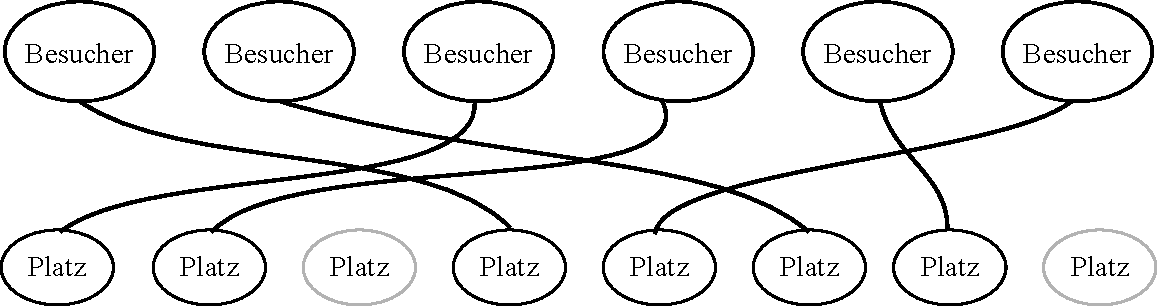
\includegraphics[scale=0.5]{Kinoabbildungen.pdf}
	\end{figure}
\end{frame}

%\begin{frame}
%	\frametitle{Lösung}
%	\textit{In dieser Teilaufgabe nehmen wir an, 6 Kinobesucher besuchten ein Kino mit 8 Plätzen. Wie viele injektive Abbildungen gibt es?} \\[2em] \pause
%	
%	Es gibt insgesamt $$8 \cdot 7 \cdot 6 \cdot 5 \cdot 4 \cdot 3 = 20160$$ injektive Abbildungen. \\[1em]
%	Der erste Besucher hat 8 Plätze zur Auswahl. Da aufgrund der Injektivität der nächste Besucher einen anderen Sitzplatz wählen muss, stehen ihm noch 7 Plätze zur Auswahl. Dies kann man für die restlichen Besucher fortsetzen.
%	
%\end{frame}

\subsection{Aufgabe 2}
\begin{frame}{Aufgabe 2}
	
	Was kann man über die Surjektivität, Injektivität und Bijektivität folgender Abbildungen sagen? Begründet jeweils kurz.
	\visible<+(-1)>{}
	\begin{alist}
		\item $f \from \R \functionto \R, \; x \mapsto x^2$ \\
		\visible<+-|handout:2->{
			Weder injektiv ($f(-2) = f(2) = 4$) noch surjektiv (auf $-1 \in \R$ wird nicht abgebildet) \impl auch nicht bijektiv.
		}
		\item $f \from \R_+ \functionto \R_+, \; x \mapsto x^2$ \\
		\visible<+-|handout:2->{
			Wir können zu jedem $y \in \R_+$ ein $x \in \R_+$ angeben, so dass $f(x) = y$, nämlich $ x = \sqrt{y}$. \\
			\impl surjektiv, und da dieses $x$ eindeutig ist auch injektiv \impl bijektiv.
		}
		
		\item $f \from \N_0 \functionto \N_0, \; x \mapsto \casesl{ 42 & \text{wenn $x = 0$} \\ x - 1 & \text{sonst} }$ \\
		\visible<+-|handout:2->{
			Nicht injektiv ($f(0) = f(43) = 42$), aber surjektiv (Für jedes $x \in \N_0$ gilt: $x + 1 \in \N_0 \text{ und } f(x+1) = x$) \\ \impl nicht bijektiv.
		} 
	\end{alist}
\end{frame}



\begin{frame}[t]
	\begin{block}{Wahr oder Falsch?}
		Sei $M$ eine beliebige endliche Menge und $f$ eine Abbildung $f \from M \functionto M$. \\
			\TrueQuestion{Wenn $f$ injektiv ist, dann ist $f$ auch surjektiv.}
			\TrueQuestion{Wenn $f$ surjektiv ist, dann ist $f$ auch injektiv.}
			\FalseQuestionE{Die beiden Aussagen gelten auch, wenn $M$ nicht endlich ist.}{Gegenbeispiele: \\ 
				$f \from \N_0 \functionto \N_0, n \mapsto 2 \· n $ \\ 
				$g \from \N_0 \functionto \N_0, n \mapsto \floor{\dfract n/2 }$}
	\end{block}
	
\end{frame}